\documentclass{UCF_ETD}
% \usepackage{times} % obsolete font package
\usepackage[T1]{fontenc}
\usepackage[utf8]{inputenc}
\usepackage{mathptmx}
\usepackage{graphicx}
\usepackage{comment}
% Files: equations.tex

%Note Inline Equations without number -- \begin{equation*} ... \end{equation*}
%Note Inline Equation with number     -- \begin{equation*} ... \end{equation}

\usepackage{amsmath}

%Unimodal Dataset Representation \cite{zong2023self}
\newcommand{\equationDu}{
\begin{equation*} \label{eq:du}
    D_u = \left\{ (x_1, y_1), (x_2, y_2), \ldots, (x_n, y_n) \right\}
    \end{equation*}
}

%Multimodal Dataset Representation \cite{zong2023self}
\newcommand{\equationDm}{
\begin{equation*} \label{eq:dm}
    D_m = \left\{ (x_{1}^{1}, \ldots, x_{1}^{k}, y_1), \ldots, (x_{n}^{1}, \ldots, x_{n}^{k}, y_n) \right\}
    \end{equation*}
}

% General Form of Contrastive Learning \cite{zong2023self} equation (9)
\newcommand{\equationGenCL}{
\begin{equation} \label{eq:genCL}
    LCon = \sum_{(r_a, r_+, r_-) \in D} \log \frac{sim(r_a, r_+)}{sim(r_a, r_+) + \sum_{j=1}^{Pm} sim(r_a, r_{-j})}
    \end{equation}
}

% General Form of Matching Prediction \cite{zong2023self} equation (10)
\newcommand{\equationGenMP}{
\begin{equation} \label{eq:genMP}
    LMatch = \frac{1}{n} \sum_{(x_{i}^{k}) \in D_m} LBCE(p_{i}, z_{i}),\text{ and } p_{i} = g_{\phi}(f_{\psi}(e_{\theta}(x_{i}^{1}, \ldots, x_{i}^{k}))),
    \end{equation}
}

\title{Collaborative Multi-Agent Framework for Multimodal Beam Prediction in 6G Networks} %Must be typed in all caps.
\author{Andrew El Kommos} % typed in all caps



\prevdegreei{M.S. University of Central Florida, 2024}
% commands available for 
% \prevdegreei{ }
% \prevdegreeii{ }
% \prevdegreeiii{ }

\thesisname{thesis}
% \thesisname prints out document type. Replace bracket text with dissertation for Ph.D students

\degreename{Master of Engineering}
% type out degree name here.

\departmentsname{Electrical Engineering}
% replace with department name if applicable.  Otherwise, do not include.

%\schoolname{Kenneth G. Dixon School of Accounting}
% replace with school name if applicable.  Otherwise, do not include.

\collegename{CECS Engineering}
% replace with college name

\termname{Spring}
% replace with semester

\termyear{2024}
% replace with year. Term year is also used to generate copyright year.

%\advisorname{Faculty Member Name with No Titles}
% replace with Major Professor if applicable.  Otherwise, do not include.


\begin{document}

\frontmatter
% applies roman numerals as page numbers

\maketitle
% prints out school info as named above

\copyrightpage{~Andrew El Kommos}


\begin{abstract}
\textit{The abstract page should be an essay-style summary of the purposes, methodology, findings or conclusions. It should not contain tables or figures of any kind. It is double-spaced. The heading ABSTRACT should be centered, without punctuation, at the top margin. If more than one page is necessary, continue on the following page. Do not repeat the heading or use the word continued.}

%% Talk about the advent of strong AI systems
The past X years have seen an large advancement in AI systems capable of solving complex tasks.

% Talking about the problems
Beam Management for millimeter wave and sub-terahertz communication systems remains a challenging task in dense urban environments. The approach of using real world sensing has attracted interested in the field of communications from both Academia and industry, which has spawned The "Multi-Modal Beam Prediction Challenge 2022: Towards Generalization" competition. This competition aims to offer a platform for investigating the viability of aligned multi-modal sensing in aiding in generalized beam management for real-world future communication systems. 


% abstract files can be added here.  I recommend using \input over \include
\end{abstract}

\dedication{I dedicate this thesis to my parents, and siblings for supporting me to continue through my education...etc}
% creates vertically and horizontally centered dedication page.  If larger than a paragraph, remove the \vspace*fil commands from the dedication section in the class file.

\begin{acknowledgments}
The acknowledgments page is optional. If you choose to use it, it should appear after the Abstract, but before the Table of Contents.
\end{acknowledgments}

\tableofcontents

\listoffigures

\listoftables

\mainmatter
% restarts page numbering with arabic numbers

\chapter{INTRODUCTION} 
% chapter headings must be typed in all caps as any \MakeUppercase command does not transfer to the PDF file through hyperref.
\textit{Chapter and major headings should be typed in all caps.  Note that Chapter titles should be formatted and positioned exactly the same as frontmatter and other major headings. However, chapters with subtitles may be stacked, single-spaced, rather than appear on one line.
The Introduction presents an overview of the thesis or dissertation material to be discussed. For sample theses and dissertations, including sample Introductions from your discipline, visit the University Writing Center’s Graduate Gateway, located at http://www.uwc.ucf.edu. Please be aware that UWC links are for content samples only, not format samples.
}

\begin{comment}
Notes and Guidance for Introduction
1. Background - Introduce readers to current state of DL/AI in communications. Talk about Evolution and Significance of real world datasets like deepsnse or others...
2. Problem Statement - Define the problem clearly -- Beam Prediction
3. Objective - Give the main objective of the thesis such as Beam Prediction and domain adaptation, using multimodal.

Multimodal Networks 
1. Theory and Significance - Discuss the role and importance of MM Networks in DL, with respect to Communications.
2. Application to Deepsense 6G -- How do MM Networks apply to dataset? Discuss how to integrate multiple types of data can enhance learning process
3. Technical Challenges of MM -- Data Fusion, synchronization, etc

Data and Communication Challenges
1. Characteristics of DeepSense Dataset - Describe data in detail -- composition, time-based measurements, etc.
2. Data Processing and Management - Challenges i`n Handling real-world data...noise filter, data cleanring, and data integrity
3. Communication Specific Challenges -- Beamforming prediction, signal interference, etc.
\end{comment}

\subsection{Background}

%Segement 1 -- Talk about the need for more advanced communication systems and their challenges....How can NN help?
Global communication networks have matured quite significanly since the first 2G mobile radio networks were deployed in the 1990s. TO support increasing network requirements for an increase user base, and throughput the communication systems will need to continue to mature. It is projected by 2030, global mobile traffic will be 670-times of the traffic in 2010, mainly due to machine-to-machine (M2M) communications. \cite{salameh20225g}\cite{ITU2370} To support this unprecedented exponential growth networks beyond 5G will need developed.


% Information about the open source models etc.
The "Deepsense 6G Dataset" is a large-scale dataset based on real-world measurements of co-existing multi-modal sensing and communication data. It compromises co-existing and synchronized multi-modal sensing and communication and is organized in a collection 
\cite{alkhateeb2023deepsense}


\subsection{Problem Statement}
% Problem statement is to define the problem clearly -- Beam Prediction

\subsection{Objectives}
% Objectives are to see what can type capabilities can be 
% enabled by applying Vision Language Models to this type of problem.
% Can we apply these type of systems, to a beacon style Agent model. 
% Applying 


\chapter{LITERATURE REVIEW}
\section{6G Communication Systems}
As modern communication systems move towards the deployment of 6G networks, the need for efficient and reliable communication systems has become increasingly important. The use of machine learning techniques in communication systems has been shown to improve the performance of wireless communication systems by optimizing the use of resources and reducing the latency of data transmission.

To address challenges in 6G communication systems novel techniques such as reconfigurable intilligence surfaces (RISs), integrated sensing and communication, mmWave and THz networks, and other methods have been proposed. \cite{zhou2023survey} Although these methods demonstrate satisfactory performance towards 6G requirements, the requirements for network management have increased in complexity and scale. The future 6G networks have leveraged machine learning (ML) as promising solution to network management techniques which optimize the use of resources and reduce the latency of data transmission. \cite{zhou2024large} To address the challenges in communication systems complexity there have been several studies that leverage techniques such as reinforcement learning \cite{zhou2021ran}, map assisted localization ray tracing techniques \cite{vuckovic2021map}, deep network assisted channel state information (CSI) prediction \cite{vuckovic2024csi}. These studies have demonstrated the potential of machine learning techniques in improving the performance of wireless communication systems. While these prior techniques demonstrate potential in improving the performance of wireless communication systems, they often rely on physics based models or simulated environments, which can fall short in capturing the complexity and variability of real-world communication systems. These limitations hinder the applicability and robustness of developed solutions, particularly in dynamic environments. To overcome these challenges, the Deepsense 6G dataset was developed to provide researches with a large-scale, real-world dataset for millimeter-wave based communication systems.  The dataset provides various sensing scenarios, such as vehicle to infrastructure, drone communication, indoor and outdoor positioning, as well as a multitude of different task sets for 6G communication applications.\cite{alkhateeb2023deepsense} The dataset provides a diverse set of scenarios and environments, which enables researchers to explore an develop deep learning networks that directly apply to real-world scenarios. In the next section, we will review the literature on the Deepsense 6G dataset and the use of deep learning techniques for millimeter-wave based communication systems.

\section{DeepSense 6G Methods}
The Deepsense 6G dataset is a real-world multi-modal dataset that provides researchers a comprehensive dataset for multi-modal sensing and communication data. The dataset provides the world's first large-scale real-world sensing and communication reprository of over a million data points, with over 30 different scenarios that target multiple applications. The team that provided the DeepSense 6G dataset aims to provide a platform that encourages the development of machine learning solutions for applications in communication systems, through a variety of multi-modal sensor technologies. There are various tasks that are supported by the dataset as well, ranging from \textit{Sensing Aided Beam Prediction} to \textit{Future Blockage Prediction}, with each task supported by a diverse set of sensing modalities. The dataset provides multiple input modalities such as GPS, Camera, Radar, and LiDAR sensing modalities aimed to enhance the breadth of the dataset for various applications. In addition to the various data points, test benches, and scenarios, the Deepsense team provides a wide array of papers, code bases, and techniques for solving problems relevant to the dataset. The inception of the DeepSense 6G dataset has marked a significant milestone in fostering research within the field of communications, particularly in scenarios requiring multi-modal sensor integration. Before the introduction of datasets like DeepSense 6G, researchers encountered substantial challenges, predominantly due to the lack of access to large-scale, realistic datasets that reflect the complexity and variety of real-world environments. \cite{alkhateeb2023deepsense}

Traditional methods for beam management often rely on exhaustive beam search techniques, which often have drawbacks in high overhead and an intractible search space. Leveraging a large-scale dataset Machine Learning frameworks are viable alternative to traditional datascience techniques as outlined in the paper, \textit{Computer Vision Aided Beam Tracking in a Real-World Millimeter Wave Deployment}. In this work the authors propose to utilize temporal visual sensing information to predict the optimal beam, as defined as the highest beamforming gain through the use of an Encoder-Decoder network. The paper presents an innovative machine learning (ML) model for beam tracking optimization in mmWave communication systems, in which a base station is equipped with an antenna array and an RGB camera to assist mobile users. The proposed model leverages visual sensing information alongside pre-defined beamforming codebooks to predict optimal future beams using an encoder-decoder architecture leveraging Recurrent Neural Networks (RNNs). The vision-aided approach demonstrates promise over the traditional methods by leveraging existing feature extraction networks to enhance beamforming gain and communication performance. \cite{jiang2022computer} The paper underscores the effectiveness of machine learning-based and vision-aided beam tracking in mmWave communications. This approach shows that it is possible to achieve a high level of accuracy for narrowing the beam search to top-5 accuracy with a precision of 99.37 percent for the next beam by observing previous time-steps on a single scenario.

\begin{figure}[h!]
  \centering
  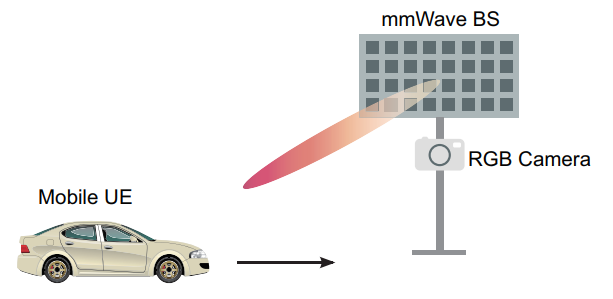
\includegraphics[width=0.5\textwidth]{Images/Literature_Review/jiang2022computer_paper.png}
  \caption{The considered system model leveraged to design a computer vision aided Beam Tracking system \cite{jiang2022computer}.}
  \label{fig:my_label}
\end{figure}

The paper's focus on next beam prediction presents limited scope, and does not take into account the some of the deeper challenges often faced in wireless communication systems by limiting it's evaluation to a single scenario. In turn the paper fails to consider the variability of real-world environments. The omission of additional sensing modalities such as radar, GPS, or other sensing inputs might limit the system's capabilites in Non-Line of Sight conditions (NLOS), where additional information might be crucial. Other methods delve into the usage of position-aided beam prediction aiming to evaluate the practicality of GPS guided predictions. In the paper \textit{Position-aided Beam Prediction in the Real World: How Useful GPS Locations Actually Are?}, the authors propose three machine learning solutions for position-aided mmWave beam prediction. They evaluate multiple methods using a Lookup Table, K-Nearest Neighbors, and a fully connected Neural network against three different scenarios. The paper reveals that the Neural Network generally outperforms both the lookup table and K-Nearest Neighbors in top-1 predictions across various scenarios due to the ability of the Neural Network to generalize better and utilize more information from training samples. They do note that factors such as input noise and label noise degrades performance and necessitates alternate metrics such as power loss, but the paper outlines the practical implications of using position data for beam alignment. Additionally, the authors point out that utilizing GPS positions can provide significant savings for the overhead of beam search in a code book that contains 64 unique codes. \cite{morais2023position}. There are several drawbacks to the use of GPS for beam alignment and some of these challenges include susceptibility to noisy inputs, latency issues, and environmental constraints, which lead the authors to suggest techniques that do not solely rely on GPS based methods. 

Location-aware methods offer a practical approach but come with limitations such as latency issues, environmental blockages, and noisy inputs. Works by the DeepSense team explore the efficacy of using Radar Aided Beam Prediction in the paper \textit{Radar Aided 6G Beam Prediction: Deep Learning Algorithms and Real-World Demonstration}. The team proposes a novel radar-aided deep learning framework to map radar samples to the optimal beam predictions. The framework leverages preprocessing of the radar samples into feature maps such as range, angle, and velocity maps using Fast Fourier Transforms (FFTs) and then employ a deep neural network subsequently to learn the mapping from the features to optimal beamforming predictions. The network is designed to be a relatively simple deep network comprosing of convolutional and fully-connected layers utilizing the rectified linear unit (ReLU) non-linear activation functions. The final layer of the network maps a hidden-layer to the designed beam code book size of 64 positions in which the objective function utilizes cross-entropy loss for predicting the optimal beam. The promise for utilizing relatively simple deep learning networks and demonstrates the capabilities of the approach showing how a the model can acheive around 90 percent for top-5 accuracy. This research underscores the potential for utilizing radar for inferring beam prediction with the radar modality. \cite{demirhan2022radar} 

\begin{figure}[h!]
  \centering
  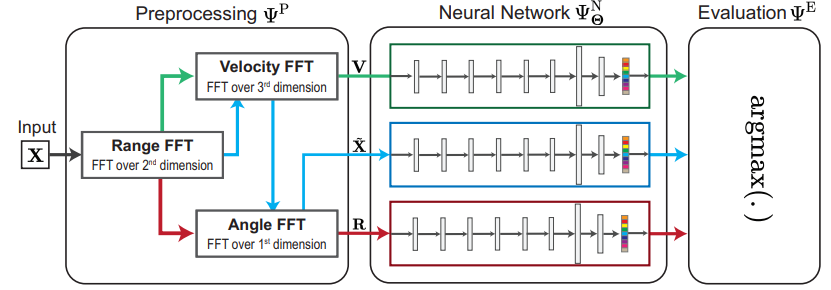
\includegraphics[width=0.5\textwidth]{Images/Literature_Review/demirhan2022radar_architecture.png}
  \caption{The considered architecture leveraged implemented in the radar aided Beam tracking paper. \cite{jiang2022computer}.}
  \label{fig:my_label}
\end{figure}

In addition to radar, vision, or position based sensing methods, other modalities like LiDAR (Light Detection and Ranging) can contibute to the diversification of environmental perception. \textit{LiDAR Aided Future Beam Prediction in Real-World Millimeter Wave V2I Communications} explores the effectiveness of utilizing LiDAR in the Beam prediction and reduction tasks. The authors argue that vision-aided methods might fall short in low light conditions, and may cause privacy concerns when it comes to positional information of the end user. The paper investigates utilizing LiDAR for mmWave beam prediction and tracking tasks, which in turn shows promising results in predicting optimal beam at 95 percent for top 5 accuracy.  

% Look at one of the multimodal papers and discuss the results and the architecture

Although these methods are effective in solving the tasks given by the dataset, they are often bespoke to the specific modalities utilized, and limited in the capabilities to adapt to different scenarios, conditions, additional tasks, and may lack the necessary requirements for real-world 6G network infrastructure. Custom designed architectures, feature engineering, task specific networks, and other drawbacks in prior deep learning methods can hinder the scalability and prohibit the widespread adoption of deep learning tehcniques to commerical 6G communication infrastructure. Ultimately, the diverse range of needed capabilities for 6G communication systems require a more general and adaptable solution that can be applied to a wide range of tasks and scenarios.

A suitable technology has emerged and potentially address these challenges. The explosion in research and commerical application of large language models (LLMs) has demonstrated the potential to solve problems in a diverse set of fields ranging from medical to financial, and have attracted significant attention in the field of communication systems. The next section will discuss the fundamentals of Large Language Models, their internal architecture, inference and utilization, and how they are utilized. 

\section{Large Language Models}

Recently, large language models (LLM) techniques have demonstrated the potential to improve through the use of massivily large models that demonstrate the ability to reason and comprehend complex tasks across various domains. The emergence of these models have shown to be effective in addressing a number of different challenges in the domains of health care, law, finance, education, and other technical fields.%\cite{Med-PaLM2, Bloomberg-GPT, etc}
 
\subsection{Large Language Model Fundamentals}
A Brief overview of the fundamentals of Large Language Models (LLMs) and their capabilities.

\subsection{Model Architecture}
The fundamental architecture of large language models is based on the transformer scheme, which utilizes an attention mechanism to capture global dependencies between inputs and outputs. 

\subsubsection{Encoder Only Architecture}

\subsubsection{Encode-Decoder Architecture}

\subsubsection{Decoder Only Architecture}

\subsection{Large Language Model Fine-Tuning}

\subsection{Large Language Models Inference and Utilization}

From early in the development of language models, natural language research such as, GPT-2 showed that LLM technologies have emergent capabilities and are unsupervised multitask learners. \cite{radford2019language}. Since this seminal paper by Radform, et. al, the field of large language models has matured significantly, and new research has emerge on how to apply the capabilities of these models across various domains and different ways. The technique of \textit(prompt engineering) is a technique that gained prominence and served as a way to improve the performance of a model by crafting input prompts. By altering the phrasing or structure of prompts, the LLM can be fine-tuned to align the behavior with a desired task. \cite{liu2023pre} The concept of In-Context learning was explored in \cite{brown2020language} and demonstrated how LLMs can adapt to new tasks by utilizing contextual clues in the input prompt. To build on the capabilities of utilizing LLMs without the need for fine-tuning, the concept of \textit(Chain of Thought reasoning) CoT was introduced in \cite{huang2023language} and demonstrates how LLMs can guided through a sequence of intermeidate reasoning steps to solve complex problems. The CoT reasoning technique demonstrated substantial improvements in solving mathematical and logical reasoning tasks by breaking down the problem into smaller steps.


\section{Multimodal Large Language Models}
% Review some literature on multimodal LLMs and Vision Language Models


\section(Large Language Model Frameworks)
% Review some literature on the frameworks that are used to train and deploy LLMs such as Hugging Face, OpenAI, Langchain, and Autogen



\section{Foundational Model's future impact on 6G Communication Systems}
% Transition into how LLMs can be used in 6G Communication Systems




\chapter{METHODOLOGY}
\section{Data Preprocessing}
The Deepsense 5G dataset compromises of data points aligned modalities using video, radar, lidar, gps, and radar.

\section{Architecture}

\section{Training Setup}

Chapter Three, also called “Methodology,” “Research Methods,” or “Research Design and Methodology,” generally presents an overview of the methods used for researching the subject.

\section{Numbering Subheadings}
All appearances of those numbered headings and subheadings, including the Table of Contents and the bookmarks, should feature exactly the same language, numbering and formatting.

\chapter{Results}
Chapter Four, also called ``Results'' or ``Data Analysis,'' usually provides detailed findings of the research.  This chapter is where tables and figures most often appear, so make sure formatting is consistent.

\section{Sample Table}
The following sample table is an example of acceptable table formatting. Descriptive titles appear above tables and may appear either on one line or stacked and single-spaced. The table itself may also be single-spaced as necessary. If at all possible, try to keep tables and/or figures all on one page. If necessary, start the table or figure on a new page, even if this means leaving blank space on the preceding page. If you must split a table over multiple pages, repeat the table headings and continue. It is not necessary to repeat the table title.

% If tables or figures are being inserted in the middle of a sentence rather than at the end of the paragraph, change the place signifier to [h!] to override LaTeX's placement.

\begin{table}[h]
\centering
\caption{Classroom Tallies}
\begin{tabular}{ |c|c|c|c|}
\hline
D & A & B & C\\
\hline
E &  3  & 4 & 7\\
\hline
F  &  5   & 8 & 9\\
\hline
\end{tabular}
\end{table}


\chapter{CONCLUSION}
Chapter Five, also called ``Summary,'' ``Conclusion,'' or ``Recommendations,'' usually presents a conclusion to the research, offers recommendations to the problem investigated, or discusses implications for future studies.

\section{Bookmarks}
A few words about bookmarks. Frontmatter entries, like the Abstract, Acknowledgments and the Table of Contents should appear in the bookmarks – but not in the Table of Contents. The TOC contains only pages that appear after the Table of Contents in the document, usually beginning with the List of Figures. So, bookmark and Table of Contents entries do vary.
However, bookmarks should include all major and chapter headings and at least first-level subheadings EXACTLY as they appear in the document (and the TOC). And readers should be able to link to pages within the ETD from all of the bookmarks, the TOC entries, as well as the Lists of Figures and Tables.
% all bookmarks are created through hyperref, so be sure that any additional packages are compatible.

\appendix

\chapter{TITLE OF APPENDIX}
\newpage
% You must include a \newpage command after each appendix.  And each appendix can be inserted as a chapter after the \appendix command.  

% This template is set to auto-letter multiple appendices.  

% If you change the secnumdepth to -1  and use multiple appendices, you must include the appendix name with the appendix title, such as APPENDIX A: TITLE.  If you have only one appendix, title it APPENDIX: TITLE.

% If you use chapter numbering and have only one appendix, you will need to comment out line 753 in the class file, containing the command \gdef\thechapter{\@Alph\c@chapter}}, and uncomment line 754 to define \gdef\thechapter{}} and remove the auto-lettering.


\noindent\labelitemi{~Begin appendix text on the page following the buffer page by using the newpage command.}\\
\labelitemi{~Continue Arabic pagination; do not restart page numbering with an appendix}\\
\labelitemi{~Use the same style and format for buffer page headings as you do for other body chapter headings.}\\
\labelitemi{~Letter, don't number, appendixes (e.g. APPENDIX A, APPENDIX B, etc.)}\\
\labelitemi{~If you have only one appendix, do not letter it at all}\\
\labelitemi{~Appendixes should follow the margin and other formatting requirements from the rest of the document}\\


\chapter{SECOND APPENDIX}
\newpage

Supplementary documentation.

\backmatter

\bibliographystyle{plain}
\bibliography{references}

\end{document}